\section{Methods}
\label{sec:methods}

This section details the computational methodologies employed to learn and utilize nonlinear deformation modes, addressing the challenges of simulating complex soft tissue behavior. We begin by laying the groundwork with a review of fundamental neural network concepts, which are central to our data-driven learning strategy. Following this, we explore the principles of subspace learning, demonstrating how neural networks can be trained to efficiently represent solutions to constrained physical problems. The core of our proposed method, the 'Neural Modes' architecture, is then introduced, including its specific design and the physics-informed loss functions crucial for its training. Finally, we describe the integration of these learned modes into dynamic simulations and discuss potential avenues for extending the framework's capabilities.



\subsection{Neural Network Principles}

A Neural Network (NN) is a mathematical model that achieves statistical generalization drawing inspiration from the human brain. Indeed, it is based on neurons, which are connected one to another, and carry the information from the input to the output \cite{Goodfellow-et-al-2016}.

It is possible to define NN as a function that maps an input to an output, given a set of parameters \( \bm{\theta} \). The function \( \hat{y} = f(\bm{x}; \bm{\theta}) \) is obtained by composing a series of functions \( f_i \) called layers, where each layer is defined as
\begin{equation}
    f_i = \sigma(W_i f_{i-1} + b_i),
\end{equation}
where \( W_i \) is the weight matrix, \( b_i \) is the bias vector and \( \sigma(\cdot) \) is the activation function. The activation function is a non-linear function that allows the network to learn complex patterns in the data. 

A neural network is trained using a dataset \( \mathcal{D} = \{(\bm{x}_i, \bm{y}_i)\}_{i=1}^N \), where \( \bm{x}_i \) is the input and \( \bm{y}_i \) is the corresponding target output. The objective is to find the optimal set of parameters \( \bm{\theta} \) that minimizes a loss function \( \mathcal{L} \), which quantifies the discrepancy between the network's predictions and the true outputs. The loss function is defined as:
\begin{equation}
    \mathcal{L}(\bm{\theta}) = \frac{1}{N} \sum_{i=1}^N L(f(\bm{x}_i; \bm{\theta}), \bm{y}_i)
\end{equation}
where \( L \) is a per-sample loss function (e.g., Mean Squared Error). The optimization process aims to find the parameters \( \bm{\theta}^* \) that minimize the overall loss:
\begin{equation}
    \bm{\theta}^* = \argmin_{\bm{\theta}} \mathcal{L}(\bm{\theta}).
\end{equation}
The optimization algorithm used is L-BFGS \cite{Liu_1989}.

The full algorithm is the following one:
\begin{algorithm} 
    \caption{Training of a neural network}
    \begin{algorithmic}
        \State Initialize the parameters \( \bm{\theta} \)
        \While{epoch < max\_epochs}
            \For{mini-batch in dataset}
                \State Perform forward pass computing \( f(\bm{x}; \bm{\theta}) \)
                \State Compute the loss function \( \mathcal{L}(f(\bm{x}; \bm{\theta}), \bm{y}) \)
                \State Perform backward pass computing the gradients of the loss function
                \State Update the parameters using the gradients
            \EndFor
        \EndWhile
    \end{algorithmic}
\end{algorithm}

\subsection{Residual Networks}

Residual Networks (ResNets), introduced by He et al. \cite{He_Zhang_Ren_Sun_2015}, are a neural network architecture designed to overcome the difficulties in training very deep networks. The core idea is the "skip connection," which allows the network to bypass one or more layers.

In a standard neural network, each layer \(f_i\) transforms the output of the previous layer \( \bm{x}_{i-1} \). A residual block, however, learns a residual function \( \mathcal{R}_i(\bm{x}_{i-1}) \). The output of the block \( \bm{x}_i \) is then the sum of the input \( \bm{x}_{i-1} \) (the skip connection) and the learned residual:
\begin{equation}
    \bm{x}_i = \bm{x}_{i-1} + \mathcal{R}_i(\bm{x}_{i-1}).
\end{equation}
The function \( \mathcal{R}_i(\bm{x}_{i-1}) \) typically consists of a few layers (e.g., two fully connected layers with activation functions).

This architecture offers several significant advantages. Primarily, it mitigates the vanishing gradient problem often encountered in deep networks. During backpropagation, gradients can flow directly through the identity skip connections, providing an alternative path that prevents them from becoming excessively small. This is evident as the gradient of a residual block's output with respect to its input includes an identity term, \( \frac{\partial \bm{x}_i}{\partial \bm{x}_{i-1}} = I + \frac{\partial \mathcal{R}_i(\bm{x}_{i-1})}{\partial \bm{x}_{i-1}} \), where \( I \) is the identity matrix. This structure ensures that even if the gradient of the residual part is small, the overall gradient is not diminished.
Furthermore, ResNets make it easier for the network to learn identity mappings. If an identity transformation is optimal for a certain part of the network, meaning the layer should ideally just pass its input through, it is simpler for the residual block to achieve this by learning a near-zero residual \( \mathcal{R}_i(\bm{x}_{i-1}) \approx \bm{0} \). This is considerably easier than compelling a stack of non-linear layers to approximate an identity function. Consequently, by addressing the vanishing gradient issue and simplifying the learning of identity or near-identity functions, ResNets enable the successful training of much deeper networks than was previously feasible, often leading to improved performance.

For our Neural Modes framework, ResNets are particularly well-suited and perform a bit better than Fully Connected Networks. We aim to learn nonlinear corrections to an existing linear modal basis. The skip connections can be thought of as preserving the input (related to the linear modes), while the residual function learns the necessary nonlinear adjustments. This aligns with our goal of enhancing, rather than completely replacing, the linear modal approximation. The architecture's ability to learn small, incremental changes is beneficial for this physics-informed correction task. 




\subsection{Neural Network Architectures}
In this work, we employ a deep residual neural network specifically designed for learning nonlinear deformation modes. This architecture builds upon traditional fully connected neural networks but incorporates residual connections to facilitate the training of deeper networks and improve performance in capturing nonlinear corrections to linear modal displacements.


\subsubsection{Neural Modes Architecture}
The Neural Modes architecture is designed to learn nonlinear corrections \( \bm{y} \) to linear deformation modes, which are parameterized by a modal coordinate vector \( \bm{z} \). A key feature of this architecture is that it ensures a zero correction output \( \bm{y}=\bm{0} \) when the input modal coordinate vector is zero \( \bm{z}=\bm{0} \), i.e., \( \text{model}(\bm{0}) = \bm{0} \). This is achieved by constructing the network entirely from layers that lack bias terms and by initializing the weights of the final output layer to zero. The specific implementation is a deep residual network, `ResidualNet', with the following structure:

\begin{itemize}
    \item \textbf{Input:} A modal coordinate vector \( \bm{z} \in \mathbb{R}^{\text{\texttt{latent\_dim}}} \), where \texttt{latent\_dim} is the dimension of the modal input space.
    \item \textbf{Network Core:}
    \begin{itemize}
        \item \textbf{Input Projection Layer:} A linear layer without bias terms that maps the input \( \bm{z} \) to a hidden representation of dimension \texttt{hid\_dim}. An activation function (default: Leaky ReLU \cite{xu2015empiricalevaluationrectifiedactivations}) is applied to the output of this projection.
        \item \textbf{Residual Blocks:} A sequence of \texttt{hid\_layers} residual blocks. Each block is designed to learn a residual function and consists of:
        \begin{itemize}
            \item Two linear layers, each without bias terms. The input to the block is first passed through a linear layer, followed by an activation function, then a Layer Normalization. This is repeated for the second linear layer and Layer Normalization within the block.
            \item Two Layer Normalization (`LayerNorm`) layers, configured without learnable affine parameters (i.e., no learnable scale or shift).
            \item An activation function (default: Leaky ReLU) applied after each linear transformation within the block, before the Layer Normalization.
            \item A skip connection that adds the input to the residual block to its processed output (after all layers in the block), facilitating gradient flow and learning.
        \end{itemize}
        \item \textbf{Output Projection Layer:} A final linear layer without bias terms that maps the processed hidden representation from the last residual block to the output correction vector \( \bm{y} \). The weights of this layer are initialized to zero.
    \end{itemize}
    \item \textbf{Output:} A nonlinear correction vector \( \bm{y} \in \mathbb{R}^{\text{\texttt{output\_dim}}} \), where \texttt{output\_dim} is the dimension of the full displacement space (e.g., number of degrees of freedom in a mesh). This correction \( \bm{y} \) is intended to be added to a linear modal displacement.
    \item \textbf{Zero-Output for Zero-Input Property:} The combined effect of using bias-free linear layers, LayerNorm without learnable affine parameters, and zero-initializing the weights of the output projection layer guarantees that if the input \( \bm{z} \) is a zero vector, the network's output \( \bm{y} \) will also be a zero vector. This is crucial for ensuring no artificial correction is applied at the rest state, aligning with physical expectations.
\end{itemize}

The network learns to map from the reduced modal space (\( \mathbb{R}^{\text{latent\_dim}} \)) to full-dimensional correction vectors (\( \mathbb{R}^{\text{output\_dim}} \)) that improve the accuracy of the linear modal approximation. This architecture, which we call Neural Modes, can be visualized as a mapping from a low-dimensional modal space to a high-dimensional displacement space, where the neural network learns to correct the linear approximation provided by the modal basis. The following figure illustrates the architecture:
% H per bloccare la figura. altrimenti metti la referenza
\begin{figure}[H]    \centering
    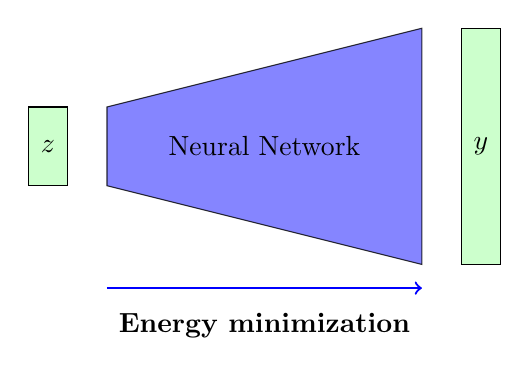
\begin{tikzpicture}
        % Modal coordinate (z)
        \draw[fill=green!20] (-3, 1) rectangle (-2.5,2);
        \node at (-2.75, 1.5) {$\bm{z}$}; % Label inside the rectangle
        
        % Displacement (u)
        \draw[fill=green!20] (2.5,0) rectangle (3,3);
        \node at (2.75, 1.5) {$\bm{y}$}; % Label inside the rectangle
        
        % Energy loss transition
        \draw[fill=blue!60,opacity=0.8] (-2,1) -- (2,-0) -- (2,3) -- (-2,2) -- cycle;
        \node at (0,1.5) {Neural Network};
        \node[below] at (0,-0.5) {\textbf{Energy minimization}};
        
        % Energy loss arrow
        \draw[thick,blue,->] (-2,-0.3) -- (2,-0.3);
    
    \end{tikzpicture}
    \caption{Neural Modes architecture for learning nonlinear deformation corrections}
    \label{fig:neural_modes_arch}
\end{figure}



\subsubsection{Training the Neural Modes} % fix this
The training process for the Neural Modes Network is based on minimizing a combination of physics-based losses, rather than simply minimizing the prediction error against ground truth data, which is the classical loss used in most neural network training. The key terms that build the loss used in training are:

\begin{enumerate}
    \item \textbf{Energy Loss}: minimizes the internal strain energy of the deformed configuration $E(\bm{X} + \bm{l} + \bm{y})$, where $\bm{X}$ is the rest position, $\bm{l}$ is the linear mode displacement given by $\bm{z}$, and $\bm{y}$ is the nonlinear correction.
    
    \item \textbf{Orthogonality Loss}: ensures that the nonlinear correction is orthogonal to the linear mode space: $\bm{y}^T \bm{l} = 0$.

    \item \textbf{Boundary Condition Penalty}: enforces the displacement boundary conditions on the deformed configuration.
    
\end{enumerate}

The total loss function is a weighted sum of these individual losses:
\begin{equation}
    \text{Loss} = \text{Energy Loss} + \lambda_1 \text{Orthogonality Loss} + \lambda_2 \text{Boundary Condition Penalty},
\end{equation}
where $\lambda_1$ and $\lambda_2$ are weight parameters that balance the importance of each loss term.

During the training process, we observed that the network had a tendency to learn a non-zero correction, even when the input modal coordinate vector was zero (\(\bm{z} = \bm{0}\)), which corresponds to the rest position of the simulated object. In an ideal scenario, the network's output should be precisely zero at this rest position, indicating that no deformation correction is necessary. This ensures that the network accurately reflects the object's behavior by only applying corrections when there are deviations from the rest state.

In the work by Wang et al. \cite{Wang_Du_Coros_Thomaszewski_2024}, an explicit origin penalty is incorporated into the loss function as a mechanism to keep the network centered around the origin. This penalty term is designed to discourage the network from learning any offset or bias that would shift its output away from zero when the input is zero. However, through our experimentation, we observed slightly better results and more stable training by adopting a bias-free network architecture. This architectural choice inherently centers the network's output at the origin, effectively achieving the same goal as an origin penalty but without the need for an additional term in the loss function.

The bias-free design ensures that the network's output is naturally centered around zero. Furthermore, this approach simplifies the loss function and potentially reduces the computational overhead during training, as it removes the need to calculate and apply an explicit origin penalty. 

During training, the Neural Modes network is optimized using a self-supervised learning approach, where the loss function is designed to minimize the internal energy of the deformed configuration while enforcing orthogonality and boundary condition constraints. Specifically, we employ the Adam optimizer to minimize a loss function that combines the energy loss with penalty terms for deviations from orthogonality and boundary conditions. The per-sample loss function \( L \) includes a Mean Squared Error (MSE) term for each constraint, ensuring that deviations are quadratically penalized. This approach allows the network to learn the underlying physics of the deformation without relying on precomputed ground truth data.


\subsection{Subspace Learning}
\begin{align}
    \label{eq:constrained_energy_minimization}
    \bm{x}^*(\phi, \psi) = \underset{\bm{x}}{\argmin} \quad & E_\phi(\bm{x}) \\
    \text{s.t.} \quad & C_\psi(\bm{x}) = 0, \nonumber
\end{align}
where \( E_\phi \) is the energy function defined by parameters \(\phi\) and \( C_\psi \) is the constraint function with parameters \(\psi\). The solution set \( \bm{x}^*\) constitutes a subspace of the full-dimensional space \( \mathbb{R}^d \). In a classical Finite Element framework, sampling from this subspace is achieved by solving a constrained minimization problem for each configuration. 

Clearly, this approach is computationally expensive, so we need a more efficient way to sample from the subspace.

The idea proposed by \cite{Wang_Du_Coros_Thomaszewski_2024} is to find a Neural Network \( \bm{x}[\theta^*](\phi, \psi) \) that approximates the solution \( \bm{x}^* \), meaning that the problem becomes:
\begin{align*}
    \bm{x}[\theta^*](\phi, \psi) \approx \underset{\theta}{\argmin} \quad & E_\phi(\bm{x}[\theta](\phi, \psi)) \\
    \text{s.t.} \quad & C_\psi(\bm{x}[\theta](\phi, \psi)) = 0.
\end{align*}

Now, defining the nonlinear modes as 
\begin{align}
    \bm{n}(\bm{z}) = \bm{l} + \argmin_{\bm{y}} \quad & E_\phi(\bm{X} + \bm{l} + \bm{y}) \\ 
    \text{s.t.} \quad & \bm{l}^T \bm{y} = 0,
\end{align}
where \( \bm{l} \) is the linear mode displacement obtained as
\begin{equation}
    \bm{l} = \sum_{i=1}^m z_i \bm{e}_i,
\end{equation}
where \( \bm{e}_i \) is the $i$-th linear mode and \( z_i \) is the corresponding modal coordinate, we can rewrite the problem \ref{eq:constrained_energy_minimization} as:
\begin{align*}
    \bm{n}[\theta^*](\bm{z}) &= \bm{l} + \bm{y}[\theta^*](\bm{z}), \\
    \theta^* = \underset{\theta}{\argmin} \quad & E_\phi(\bm{X} + \bm{l} + \bm{y}[\theta](\bm{z})) \\
    \text{s.t.} \quad & \bm{l}^T \bm{y}[\theta](\bm{z}) = 0.
\end{align*}

Now we define a suitable function that will serve as a loss function for the self-supervised training of the neural network. The loss function is defined as:
\begin{equation}
    \mathcal{L}(\theta) = \mathbb{E}_{\bm{z}} \left[ E(\bm{X} + \bm{l} + \bm{y}[\theta](\bm{z})) + \lambda_1 \bm{l}^T \bm{y}[\theta](\bm{z}) + \lambda_2 \text{B. C. Penalty} \right],
\end{equation}
where \( \lambda_1 \) and \( \lambda_2 \) are hyperparameters that control the importance of the orthogonality and boundary condition penalty terms, respectively. The first term is the energy loss, which minimizes the internal strain energy of the deformed configuration, while the second term ensures that the nonlinear correction is orthogonal to the linear mode space. The third term enforces the displacement boundary conditions on the deformed configuration.

\subsection{Sampling the Modal Space}
One of the main challenges for this method is finding a good way to sample the \(z\) vector that will be used as input for the neural network. Here are two examples that shows how choosing randomly the \(z\) vector can lead to unrealistic results. 
\begin{figure}[H]
    \centering
    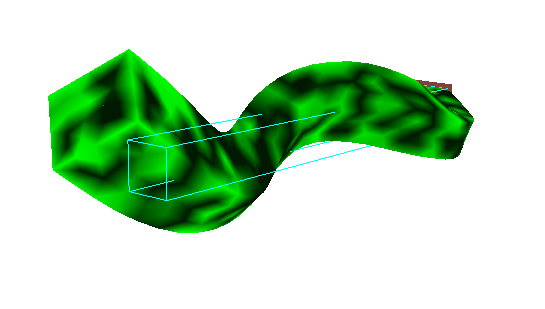
\includegraphics[width=0.4\textwidth]{Images/z_random.png}
    \caption{Example of a bad sampling of the modal space, the reference shape is the light blue outline.}
    \label{fig:bad_sampling}
\end{figure}
In this example, the random \(z\) vector has large values in its latter components. These components represent higher-frequency deformation modes, which naturally contain more strain energy. Using these modes with high amplitudes often creates physically unrealistic or extreme configurations. This shows why random sampling across all components of \(z\) can lead to unrealistic deformations.

A better sampling approach considers the physical meaning of each mode. The first components of \(z\) typically correspond to lower-frequency, global deformation modes that represent major shape changes with less energy. Later components represent higher-frequency, localized, and more energetic modes. 

For more effective sampling of the modal space, we can implement a strategic approach to generating the \(z\) vectors. This approach involves assigning larger coefficient values to the first several components of the vector, which typically correspond to the fundamental, lower-frequency deformation modes, while progressively reducing the magnitude of values assigned to later components. By structuring our sampling in this manner, the resulting deformations tend to be significantly more physically realistic and energetically feasible in real-world scenarios. This methodical sampling focuses the neural network's training process on common, naturally occurring deformation patterns rather than directing computational resources toward unlikely, high-energy configurations that rarely manifest in practical applications.

The fundamental issue with purely random sampling across all modal coordinates is that it inadvertently forces the neural network to attempt energy minimization for physically implausible states. Given that the energy landscape for soft tissue deformation is already inherently complex and high-dimensional, introducing this additional unnecessary complexity substantially increases the difficulty of the training process and potentially compromises the quality of the learned model. This consideration underscores the necessity for developing a more sophisticated and physically-informed strategy to efficiently sample the modal space, allowing the network to concentrate on learning the most relevant aspects of the deformation behavior.


\subsection{Dynamic Simulation with Neural Modes}
For dynamic simulations, the Neural Modes framework solves an optimization problem at each time step. Given the current and previous displacement states $\bm{u}_n$ and $\bm{u}_{n-1}$, the modal coordinates for the next time step $\bm{z}_{n+1}$ are computed by:
\begin{equation}
    \bm{z}_{n+1} = \underset{\bm{z}}{\argmin} \frac{1}{2h^2} \|\bm{n}(\bm{z}) - 2\bm{u}_n + \bm{u}_{n-1}\|_{\bm{M}}^2 + E(\bm{n}(\bm{z})),
    \label{eq:optimization_problem}
\end{equation}
where $\bm{n}(\bm{z})$ represents the complete displacement field (linear modes plus nonlinear correction), $h$ is the time step, $\bm{M}$ is the mass matrix, and $E(\cdot)$ is the internal energy of the configuration. This optimization problem is typically solved using the L-BFGS-B algorithm \cite{Liu_1989}.

One challenge with this approach is that the optimization problem does not explicitly account for external forces. The network learns to minimize internal energy but lacks direct information about external forces that may be applied during simulation: this limitation can affect the accuracy of dynamic simulations, particularly for large deformations or complex loading conditions.



\subsection{Modal Forces}

To validate the Neural Modes framework and generate physically meaningful training data, we employ a modal force generation approach that leverages the principal deformation modes of the mechanical system. This method addresses the challenge of creating external forces that produce representative deformations while maintaining the nonlinear capabilities essential for large deformation scenarios \cite{odotDeepPhysicsPhysicsAware2021}.

\subsubsection{Mathematical Derivation and Linearization Process}

The foundation of our modal force approach lies in the linearization of the nonlinear finite element equilibrium equations. Starting from the weak form of the hyperelastic boundary value problem, we seek displacement $\bm{u}$ such that:
\begin{equation}
    \int_{\Omega} \bm{P}(\bm{u}) : \nabla \bm{w} \, d\Omega = \int_{\Omega} \bm{f} \cdot \bm{w} \, d\Omega + \int_{\Gamma_N} \bm{h} \cdot \bm{w} \, d\Gamma \quad \forall \bm{w} \in V,
\end{equation}
where $\bm{P}(\bm{u})$ is the first Piola-Kirchhoff stress tensor, $\bm{f}$ represents body forces, and $\bm{h}$ are traction forces on the Neumann boundary $\Gamma_N$.

In the finite element discretization, this leads to the nonlinear system:
\begin{equation}
    \bm{R}(\bm{u}) = \bm{f}^{int}(\bm{u}) - \bm{f}^{ext} = \bm{0},
\end{equation}
where $\bm{f}^{int}(\bm{u})$ are the internal forces (functions of displacement) and $\bm{f}^{ext}$ are the external forces. The residual vector $\bm{R}(\bm{u})$ represents the out-of-balance forces.

To solve this nonlinear system, we employ the Newton-Raphson method \cite{Dedieu_2015}, which requires linearization around the current configuration $\bm{u}^k$:
\begin{equation}
    \bm{R}(\bm{u}^k + \Delta\bm{u}^k) \approx \bm{R}(\bm{u}^k) + \frac{\partial \bm{R}}{\partial \bm{u}}\bigg|_{\bm{u}^k} \Delta\bm{u}^k = \bm{0}.
\end{equation}

The tangent stiffness matrix is defined as:
\begin{equation}
    \mathbb{K}(\bm{u}^k) = \frac{\partial \bm{R}}{\partial \bm{u}}\bigg|_{\bm{u}^k} = \frac{\partial \bm{f}^{int}}{\partial \bm{u}}\bigg|_{\bm{u}^k},
\end{equation}
leading to the linearized system at each Newton iteration:
\begin{equation}
    \mathbb{K}(\bm{u}^k) \Delta\bm{u}^k = -\bm{R}(\bm{u}^k) = \bm{f}^{ext} - \bm{f}^{int}(\bm{u}^k).
\end{equation}

For our modal force generation, we consider the linearization at the rest configuration $\bm{u}^0 = \bm{0}$, where the internal forces vanish: $\bm{f}^{int}(\bm{0}) = \bm{0}$. This simplifies the linearized system to:
\begin{equation}
    \mathbb{K}(\bm{0}) \Delta\bm{u}^0 = \bm{f}^{ext}.
\end{equation}

\subsubsection{Modal Decomposition and Force Generation}

The tangent stiffness matrix at the rest configuration $\mathbb{K} = \mathbb{K}(\bm{0})$ can be decomposed using eigenvalue analysis:
\begin{equation}
    \mathbb{K} = \boldsymbol{\Phi} \boldsymbol{\Lambda} \boldsymbol{\Phi}^T,
\end{equation}
where $\boldsymbol{\Phi} = [\bm{\phi}_1, \bm{\phi}_2, \ldots, \bm{\phi}_n]$ contains the eigenvectors (deformation modes) and $\boldsymbol{\Lambda} = \text{diag}(\lambda_1, \lambda_2, \ldots, \lambda_n)$ contains the corresponding eigenvalues.

From the linearized equilibrium equation, we can express:
\begin{align}
    \mathbb{K} \Delta\bm{u}^0 &= \bm{f}^{ext} \\
    \boldsymbol{\Phi} \boldsymbol{\Lambda} \boldsymbol{\Phi}^T \Delta\bm{u}^0 &= \bm{f}^{ext} \\
    \boldsymbol{\Phi} (\boldsymbol{\Lambda} \boldsymbol{\Phi}^T \Delta\bm{u}^0) &= \bm{f}^{ext}.
\end{align}

Defining the modal coefficients as $\bm{q} = \boldsymbol{\Lambda} \boldsymbol{\Phi}^T \Delta\bm{u}^0$, we obtain:
\begin{equation}
    \bm{f}^{ext} = \boldsymbol{\Phi} \bm{q}.
\end{equation}

This fundamental relationship allows us to generate external forces by selecting appropriate modal coefficients $\bm{q}$. Each component $q_i$ represents the amplitude of the $i$-th deformation mode in the applied force pattern.


The modal force generation methodology offers several significant advantages that directly support the development and validation of our Neural Modes framework. First, the approach ensures physical meaningfulness in the generated test cases. Since the forces are derived from the principal deformation patterns of the mechanical system, the resulting displacements naturally exhibit the characteristic behavior of the material under consideration. This is particularly important for soft tissue simulation, where unrealistic deformation patterns can compromise the validity of the learned model.

The method also provides controlled deformation generation capabilities. By systematically selecting specific combinations of modal coefficients $\bm{q}$, we can generate comprehensive datasets that span the most significant deformation modes of the system. This systematic approach allows us to ensure adequate coverage of the deformation space while avoiding the computational expense of exhaustive sampling. The ability to control the relative contributions of different modes enables us to focus the training process on the most relevant aspects of the mechanical behavior.

Furthermore, the modal force approach preserves material properties throughout the generation process. Since the modal basis is directly derived from the material's stiffness matrix, which incorporates the constitutive relationships and geometric configuration, the generated forces inherently respect these fundamental characteristics without requiring manual calibration or parameter tuning. This automatic consistency reduces the likelihood of introducing artifacts or bias in the training data.

Despite utilizing linear modal analysis for force generation, the framework retains full nonlinear capability in the solution process. The modal decomposition serves only to structure the external loading; the actual deformation computation employs the complete nonlinear finite element formulation, preserving all geometric and material nonlinearities. This approach allows us to leverage the computational efficiency of modal analysis while maintaining the accuracy required for large deformation scenarios.

Finally, modal forces provide an ideal validation framework for the Neural Modes network. Since we possess analytical knowledge of the modal responses and can systematically vary the input conditions, we can rigorously assess the network's ability to capture both the linear modal behavior and the nonlinear corrections. This controlled environment enables us to verify that the learned corrections indeed improve upon the linear modal approximations and to identify potential limitations or areas for improvement in the network architecture or training process.

For validation purposes, we generate test cases by sampling the modal coefficient vector $\bm{q}$ and computing the corresponding full nonlinear deformation using finite element analysis. The Neural Modes network's ability to reproduce these deformations accurately demonstrates its effectiveness in capturing the nonlinear behavior while leveraging the underlying modal structure.

This modal force approach also facilitates the generation of training data that focuses on the most energetically favorable deformation patterns, complementing the strategic sampling of modal coordinates discussed earlier. By ensuring consistency between the force generation and the modal coordinate sampling, we create a coherent framework for both training and validation of the Neural Modes network.

